% ===========================================================================
\section{Air-Pollutant Co-Emissions}
\label{sec:air}
% ===========================================================================

Open municipal-waste burning uses the same wet/dry burned quantity and fate account as the greenhouse-gas calculation. The FY2023--24 reference burned mass is \SI{9.40}{\mega\tonne}; pollutant-specific garbage-burning factors follow \citet{andreae2019}. Masses are reported in native units. Burning locations are not observed nationally, so the population allocation describes waste origin rather than confirmed release sites.

\begin{table}[htbp]
\centering
\footnotesize
\begin{tabular}{@{}lr@{}}
\toprule
\textbf{Pollutant} & \textbf{kt/yr} \\
\midrule
CO                  & 434.45 \\
NMVOC               & 151.40 \\
\PM{}               &  63.85 \\
HCl                 &  18.43 \\
\NOx{} (as NO$_2$)  &  15.14 \\
Black carbon        &   9.22 \\
\NHthree{}          &   5.92 \\
\SOtwo{}            &   3.29 \\
\bottomrule
\end{tabular}
\caption{Air pollutants from open waste burning, FY2023--24. Mass only; these never enter a
greenhouse-gas total. Computed from the same burned tonnage as the 4C2 emissions above, so the
two describe the same fire. \NOx{} is reported as NO$_2$-equivalent
(Andreae publishes the garbage-burning factor as NO; the conversion is documented on the
factor row), the inventory-wide basis.}
\label{tab:air}
\end{table}

\begin{figure}[htbp]
\centering
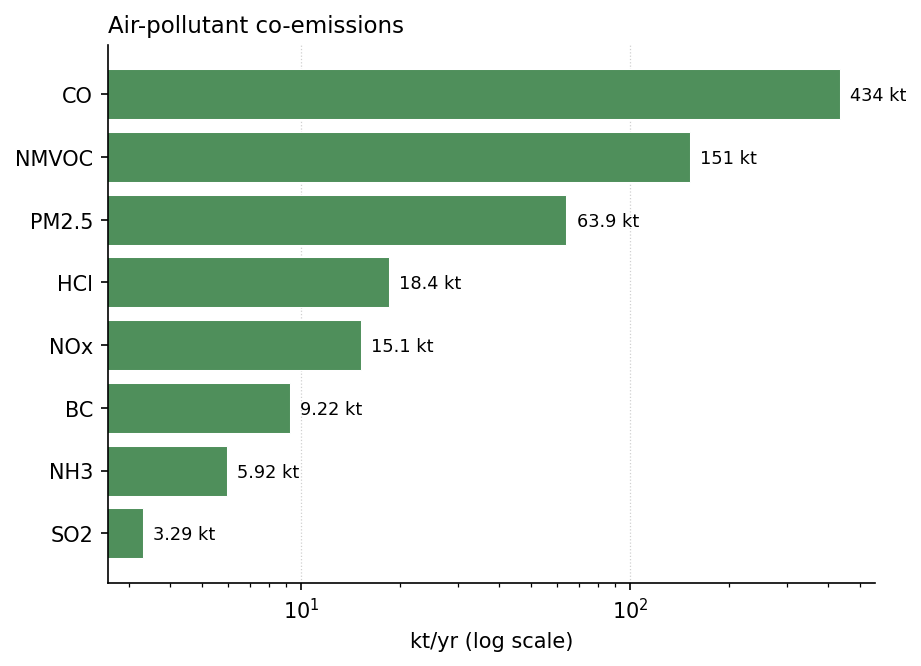
\includegraphics[width=\linewidth]{waste_air.png}
\caption{The same figures on a log axis, which the range demands: carbon monoxide and
sulphur dioxide differ by more than two orders of magnitude, and a linear axis renders
everything below \PM{} as a line of zero width.}
\label{fig:air}
\end{figure}

\subsection{Interpretation of primary particulate releases}

The reference estimate is \SI{63.85}{\kilo\tonne} of primary PM$_{2.5}$. Its relative contribution depends on the compared pollutant, source coverage and household or industrial configuration. No inverse relationship between GHG and pollutant rankings is assumed. Emitted mass does not establish exposure: disposal and burning locations, release conditions, atmospheric transport and chemistry remain outside this calculation.

The common activity account prevents disposal and burning from claiming the same generated waste twice. It does not establish where the uncollected material burns or validate the pollutant factors. The unburned uncollected fraction remains an unresolved fate, rather than an invented combustion destination.

\subsection{Black carbon and hydrogen chloride}

Two entries deserve comment because they are specific to waste rather than generic to
combustion.

Black carbon at \SI{9.22}{\kilo\tonne} is a strong short-lived warming agent that this
inventory reports as mass and does not convert to \COe{}, following the convention that its
metrics remain contested. It is reported because omitting it would understate the climate
relevance of open burning even while the greenhouse-gas total for 4C2 is small.

Hydrogen chloride at \SI{18.43}{\kilo\tonne} appears in no other sector of this inventory and
is a direct consequence of burning chlorinated plastics in the open. It does not quantify dioxin or furan releases, which require separate source-specific methods.

\subsection{Limitations of this layer}

The conditional air ensemble reuses the same bounded waste-fate realisations as the GHG calculation, then applies pollutant-factor uncertainty. Burning-fraction alternatives remain separate structural cases; their endpoints are not confidence limits. The composition is regional rather than Pakistani, which matters more for
pollutants than for greenhouse gases because plastics and textiles drive the chlorine and much
of the particulate. And the factors describe open burning generically rather than the specific
conditions of Pakistani street-side burning---smouldering, damp, and often mixed with organic
waste---whose consequences for incomplete-combustion products require local evidence.
